\section{Introducción}

\hrule
\vspace{5mm}
\\
La tiroides es una glándula pequeña situada en la parte anterior del cuello, encargada de la producción de dos hormonas tiroideas: la tiroxina (T4), que 
<<<<<<< HEAD
corresponde al 93 por ciento de hormona secretada por la glándula tiroides, y la 3,5,3-triyodotironina (T3) \cite{Stegmann} . Dicha glándula regula procesos metabólicos esenciales, tanto en la etapa de desarrollo, como en la edad adulta. Estos procesos están relacionados con el metabolismo energético, incrementando el consumo calórico, regulando el crecimiento y maduración de los tejidos y el recambio de prácticamente todos los sustratos, vitaminas y hormonas.  \cite{Stegmann} 
\\ \\
El término tiroiditis (HP:0100646) se asocia con todas aquellas enfermedades que presentan inflamación de la glándula tiroides \cite{Sweeney2014}. Los síntomas que produce la tiroiditis varían dependiendo de la enfermedad tiroidea que la produzca. No obstante, podemos diferenciar dos efectos diferenciados provocados por la tiroiditis \cite{Pulgarin} : 
=======
corresponde al 93 por ciento de hormona secretada por la glándula tiroides, y la 3,5,3-triyodotironina (T3) \cite{Stegmann} . Esta regula procesos metabólicos esenciales tanto en la etapa de desarrollo como en la edad adulta. \cite{Stegmann} 
\\ \\
El término tiroiditis (HP:0100646) se asocia con todas aquellas enfermedades que presenten inflamación de la glándula tiroides \cite{Sweeney2014}. Los síntomas que produce la tiroiditis variarán dependiendo de la enfermedad tiroidea que la produzca. No obstante, podemos diferenciar dos efectos diferenciados provocados por la tiroiditis \cite{Pulgarin} : 
>>>>>>> af19c8c0bd0178706be517ccd733e33c981467ab
\begin{itemize}
    \item Hipotiroidismo. Condición en la cual la glándula tiroides no puede producir la suficiente cantidad de hormonas tiroideas necesarias para cumplir con el requerimiento tisular.
    \item Hipertiroidismo. Incremento sostenido de las hormonas tiroideas debido al aumento de biosíntesis y secreción de la tiroides.
\end{itemize} 
\\ \\
<<<<<<< HEAD
\vspace{5mm}
Entre las enfermedades más conocidas que presenten tiroiditis tenemos la enfermedad de Hashimoto 'HT' (HP:0000872). Siendo la característica más común una elevación de los anticuerpos autoinmunes TPOAb y TGAb en las celulas tiroideas. HT estando presente aproximadamente en el 5 por ciento de la población mundial, siendo actualmente la enfermedad autoinmune con mayor incidencia \cite{Zheng2020}. Principalmente su sintomatología es bocio no-doloroso, hipotiroidismo y elevación de TPO \cite{Sweeney2014}. A su vez, encontramos una alta comorbilidad de HT con la diabetes tipo 1, Turner syndrome, Addison disease, y hepatitis C no tratada.\cite{Sweeney2014} 
Existen otros subtipos menos comunes de la tiroiditis, tales como tiroiditis infecciosa, tiroiditis post-parto o tiroiditis inducida por radiación. \cite{Sweeney2014}  
\vspace{20mm}

\\ \\
Diversos factores  intervienen en el desarrollo de enfermedades relacionadas con la tiroiditis: factores genéticos, factores ambientales (infecciones producidas por agentes externos), dietéticos (relacionados con los niveles de ingesta de yodo) o de otro tipo como el estrés, el tabaquismo o incluso el embarazo. Destacan los genéticos, siendo los de mayor implicación en este tipo de enfermedades. \cite{Hiromatsu}
\\ \\ 
Hasta la fecha se han encotrado un total de 46 genes asociados a la tiroiditis \cite{StringHP:0100646}. Aquellos genes con mas relaciones registradas son: el HLA-DR, los genes inmunorreguladores (CD40, CTLA-4, PTPN22, FOXP3 y CD25) y los genes específicos del tiroides (tiroglobulina [TG] y receptor de la hormona tiroestimulante [TSH]).
Estos, principalmente, están relacionados con dos procesos moleculares: la unión de proteínas y péptidos y con la actividad de los receptores inmunes. \cite{Hiromatsu}
\\ \\
En relación a los genes implicados en la unión de proteínas y péptidos; se encuentran involucrados en la regulación de citoquinas (SOCS1) y en el crecimiento celular, así como en la  apoptosis (PIK3CA) y en la supervivencia celular inducida por daño al ADN (PRKCD). Estando estos procesos inmiscuídos tanto en la propia fisiología de la tiroiditis, como en enfermedades autoinmunes o cáncer.\cite{StringHP:0100646, Yamada2022, PRKCDGeneCards}
\\ \\ 
Entre los genes asociados a la actividad de los receptores inmunes (actividad involucrada en el inicio de la respuesta inmune a partir de la recepción y transmisión de señales entre células) encontramos: IL2RG, IL7R, IL2RA, HLA-DQB1 y HLA-DQA1. Destacan la familia HLA  perteneciente al complejo MHC (Major histocompatibility complex), ya que juegan un papel fundamental en el sistema inmunológico presentando péptidos de proteínas extracelulares. \cite{HLA}Así como la familia de ILR, compuesta por IL2RG, IL7R y IL2RA. Estos genes son los responsables de la producción de receptores de citoquinas, participando en la regulación de la tolerancia inmune mediante el control de células T. \cite{StringHP:0100646}
\\ \\ \newpage
En la siguiente imagen podemos ver la red de genes relacionados con el fenotipo tiroiditis (HP:0100646), siendo representados de azul aquellos que intervienen en la actividad de los receptores inmunes, de rojo los que intervienen en la unión de péptidos y bicolor los que intervienen en ambas.
\vspace{5mm}
=======
Entre las enfermedades más conocidas que presenten tiroiditis tenemos la enfermedad de Hashimoto (HT). Es conocido que alredeor del 20-30 por ciento de la población sufre de HT. \cite{Zheng2020}. Principalmente la sintomatologia de HT es bocio-no doloroso, hipotiroidismo y elevación de TPO \cite{Sweeney2014}. A su vez existen otros subtipos tales como tiroiditis infecciosa, tiroiditis post-parto o tiroiditis inducida por radiación. \cite{Sweeney2014}
\\ \\
 Diversos factores  intervienen en el desarrollo de estas enfermerdades, como por ejemplo los factores de tipo ambiental (infecciones producidas por agentes externos), factores dietéticos (relacionados con los niveles de ingesta de yodo) u otro tipo de factores como el estrés, el tabaquismo o incluso el embarazo. \cite{Hiromatsu}
\\  \\ 
 Por ejemplo, hablando de la enfermedad de Hashimoto, el 50 por ciento de los factores que producen dicha enfermedad son genéticos, por lo que nos encontramos ante aquellos factores de mayor implicación. Siendo la característica más común, una elevación de los anticuerpos autoinmunes TPOAb y TGAb en las celulas tiroideas.\cite{Zheng2020} A su vez se ha encontrado una alta coexistencia de HT con la diabetes tipo 1, Turner syndrome, Addison disease, and  hepatitis C no tratada.\cite{Sweeney2014}
\\ \newpage
Hasta la fecha varios genes se han asociado al fenotipo, como el HLA-DR, los genes inmunorreguladores (CD40, CTLA-4, PTPN22, FOXP3 y CD25) y genes específicos del tiroides (tiroglobulina [TG] y receptor de la hormona tiroestimulante [TSH]), siendo estos son los más citados; no obstante, encontramos un total de 46 genes asociados al fenotipo. 
\\ \\
Estos genes principalmene están relacionados con dos procesos moleculares: la unión de proteínas y péptidos (importante en la estructura del cromosoma) y en la actividad de los receptores inmunes. Dicha actividad consiste en recibir señales y transmitirlas a células para iniciar una respuesta inmune en éstas.
\cite{Hiromatsu}
En la actividad de los receptores inmunes, están implicados los genes IL2RG, IL7R, IL2RA, HLA-DQB1 y HLA-DQA1. Podemos destacar estos dos últimos, siendo ambos pertenecientes a la clase MHC (Major histocompatibility complex). Ambos genes juegan un papel fundamental en el sistema inmune ya que presentan aquellos péptidos de proteínas extracelulares. \cite{HLA} 
\\ \\
Sin embargo,los genes restantes no se encargan de la unión de proteínas, pues encontramos varios que no participan en ninguno de los dos procesos moleculares. Destacar que  la familia de ILR, compuesta por IL2RG, IL7R y IL2RA , participan en ambos procesos, por lo que podemos afirmar que son de gran importancia en la tiroiditis. 

En la siguiente imagen podemos ver la red de genes relacionados con nuestro fenotipo, siendo representados de azul aquellos que intervienen en la actividad de los receptores inmunes, de rojo los que intervienen en la unión de péptidos y bicolor los que intervienen en ambas.
>>>>>>> af19c8c0bd0178706be517ccd733e33c981467ab
\begin{center}
 
    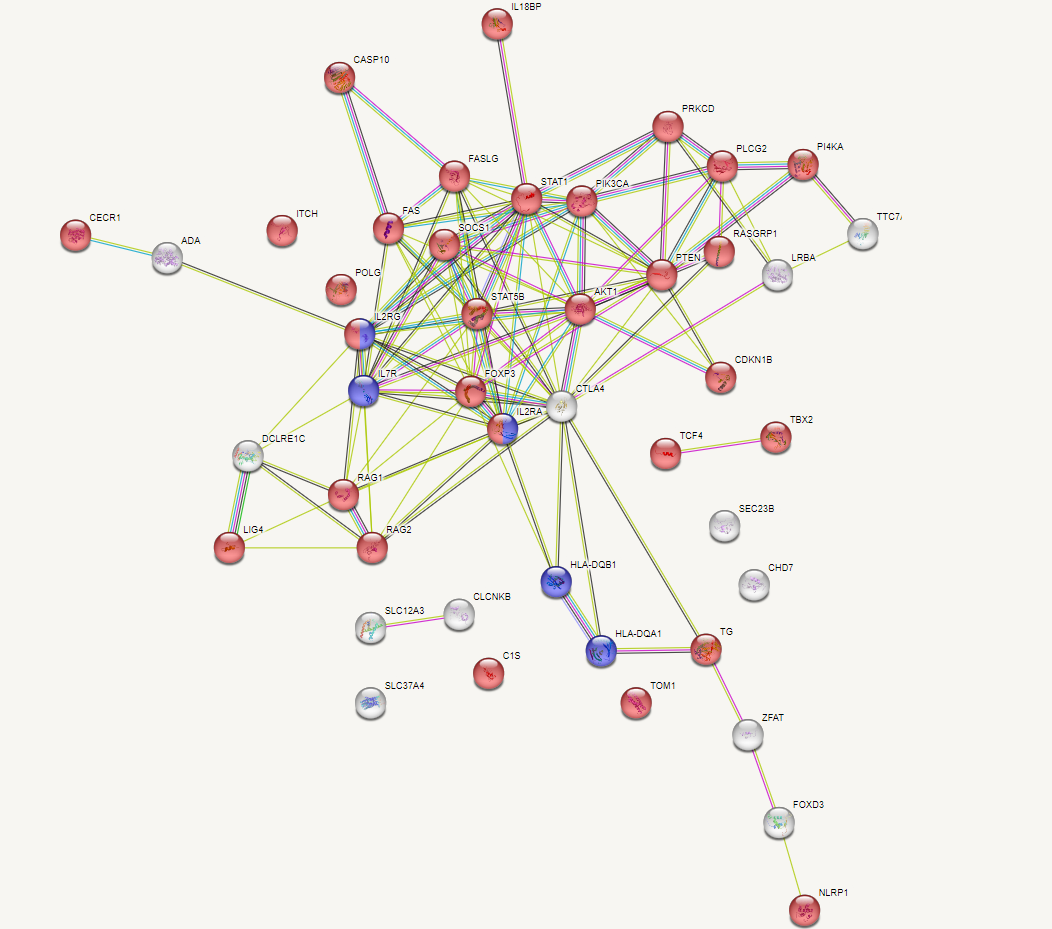
\includegraphics[scale=0.4]{figures/red de genes.png}
    
<<<<<<< HEAD
    Figure 2.1. Red de Genes HP:0100646
\end{center}
\\ \\ 
\vspace{5mm}
Los factores genéticos constan de una gran importancia en las enfermedades relacionadas con la tiroiditis, aunque en HT tienen especial relevancia, estando asociados al origen del 50 por ciento de los casos.\cite{Zheng2020} Encontramos 17 genes asociados a la enfermedad de Hashimoto. Algunos de estos genes (PTEN, PLCG2, CTLA4, TTC7A) se han encontrado involucrados en la enfermedad inflamatoria intestinal, con fisiología autoinmune. No obstante, existe una carencia de información sobre los procesos moleculares y las relaciones entre los genes involucrados en HT. Siendo estas mayormente obtenidas a partir de textmining sobre estudios de enfermedades no tiroideas con fisiología autoinmune. \cite{StringHP:0000872}
\\ \\  
Dada la importancia de los factores genéticos en la tiroiditis y del gap de conocimiento identificado en HT, el estudio se centra en la realización de un análisis de los diferentes genes asociados a dichos fenotipos y de las funciones moleculares en los que estan asociados. Para la identificación de nuevas relaciones genéticas y procesos moleculares asociados se tiene en cuenta el tipo de interacción (física, co-expresión, databases, etc...) entre los genes involucrados, así como las funciones moleculares compartidas por ambos.





=======
    Figure 2.1. Red de Genes
\end{center}
\\ \\
Dada la importancia de los factores genéticos en este fenotipo (HP:0100646), el estudio se centrará en la realización de un análisis de los diferentes genes asociados a dicho fenotipo y de las relaciones funcionales entre estos. 
\\ \\  \newpage 
Se tendrán en cuenta el tipo de interacción (física, co-expresión, databases, etc...) a partir de las cuales diluciar los diferentes clusters. Estos clusters ayudarán a clasificar genes en base a la función molecular que desempeñen. La distribución de genes resultante ayudará a descubrir cuales de ellos tienen una mayor relevancia.
\\ \\
>>>>>>> af19c8c0bd0178706be517ccd733e33c981467ab




